\section{Data and Evaluation Protocol}
\label{sec:data}
\paragraph{Data}
The training set contains 100 patients, 20 per group; the test set contains 50 patients, whose labels are hidden. For each patient, we have the short-axis MRI volumes at ED and ES, their segmentations (background, RV, myocardium, LV), the height and the weight. Volumes have 6 to 21 slices, with a slice step of 5 to 10 mm and an in-plane resolution of about 1.5 mm (Appendix~\ref{app:data}). Figure~\ref{fig:data} shows one patient per group. In the test segmentations, the LV cavity is labeled as background: it has to be reconstructed before any LV volume can be computed. Our code ignores any LV label found in a test file and never writes to the data folders, so the pipeline always starts from the data as distributed.

\begin{figure}[!htb]
  \centering
  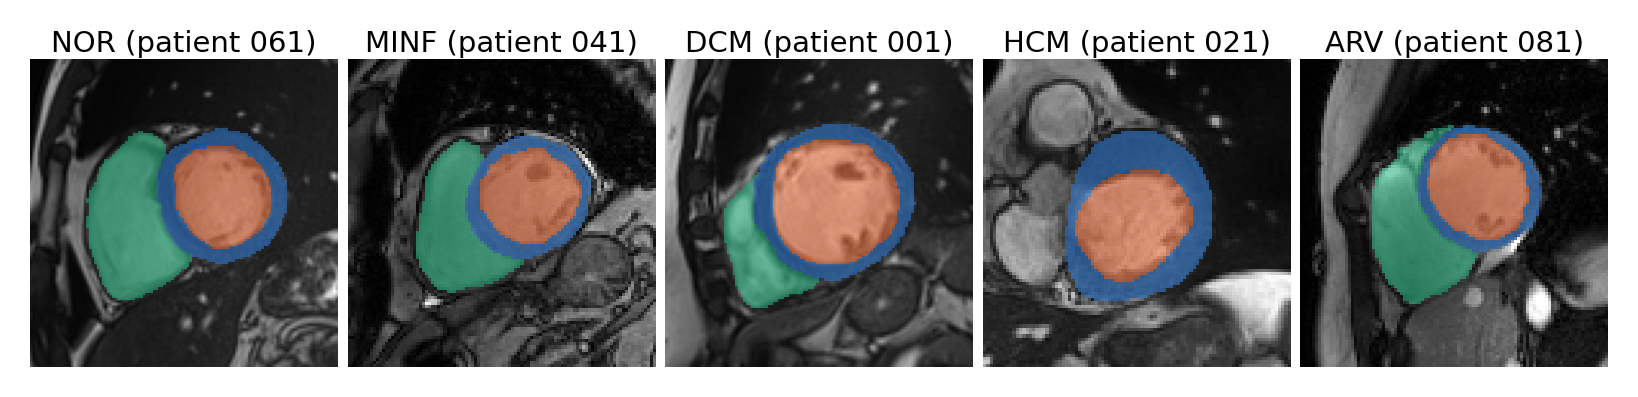
\includegraphics[width=\linewidth]{figs/data_overview.png}
  \caption{Mid-ventricular slice at end-diastole of the first training patient of each group, with the segmentation: RV (green), myocardium (blue), LV cavity (orange).}
  \label{fig:data}
\end{figure}

\paragraph{No data augmentation}
Geometric augmentation of the masks (rotations, translations, flips) is of no use for this task: all our features are measured in millimeters on the segmentations and are invariant to these transformations. A zoom that does not update the voxel spacing would change the volumes without changing the label, and would therefore add label noise. We do not augment the data.

\paragraph{Protocol}
All accuracies of this report are estimated by nested cross-validation \citep{varma2006}. The outer loop is a stratified 5-fold cross-validation, repeated 10 times with different shuffles; every patient receives one out-of-fold prediction per repeat. Inside each training fold, a stratified 5-fold cross-validation selects the hyper-parameters, and the feature scaling is fitted on the training fold only. We report the mean and standard deviation of the accuracy over repeats. Classes are balanced, so the balanced accuracy equals the accuracy; macro-F1 and per-class recalls are in Appendix~\ref{app:bench}. All configurations use the same outer splits, so we also report their paired difference with the best configuration. The standard deviation over repeats ignores the variability due to the sample itself \citep{nadeau2003}: with 100 patients, differences of one or two points should not be over-interpreted.

\paragraph{Implementation}
The code is a Python package and six scripts (indexing, LV reconstruction, features, protocol study, benchmark, final model), built on scikit-learn \citep{pedregosa2011}, PyTorch \citep{paszke2019}, SciPy, scikit-image and XGBoost \citep{chen2016}. Every run records its configuration, library versions, metrics, tables and figures (Appendix~\ref{app:runs}). Everything runs on an Apple M3 laptop in about 1 hour and 30 minutes, most of it spent training MLP ensembles inside the nested cross-validation.
